\chapter{Problem Statement}
\label{ch:problem}

\section{Problem context}
Restaurant recommenders are usually built to predict ratings from past user--item
interactions \citep{koren2009matrix}. Review-based recommenders add review text, but most
still use it to improve rating prediction rather than to answer a new free-text request
\citep{hasan2025reviewsurvey}. This leaves three gaps for a diner who types a request such as
``I am on a budget'':
\begin{enumerate}
  \item \textbf{Query matching.} The system must connect the user's words to the words of
  reviewers. A user who writes ``affordable'' should also find reviews that say ``cheap'' or
  ``good value''.
  \item \textbf{Evidence.} The system should show why a restaurant was chosen, and the reason
  should be checkable against the original reviews.
  \item \textbf{Language.} The method should work for Thai reviews as well as English ones,
  even though Thai has no spaces between words and taste words are often written informally
  (\thai{แซ่บ}, \thai{เผ็ดดดด}).
\end{enumerate}

\section{Task definition}
Let $R$ be a set of restaurants and $q$ a free-text query. Each restaurant $r \in R$ is
represented by a set of text units $U_r$, where a unit is either a whole review or a single
review sentence. A retrieval model assigns a score $s(q,u)$ to every unit $u$. For BM25 this is
the lexical relevance score \citep{robertson2009bm25}; for the dense model it is the cosine
similarity between the query and unit embeddings \citep{reimers2019sbert}. The restaurant score
is an aggregation of the unit scores:
\begin{equation}
  S(q,r) = f\big(\{\, s(q,u) : u \in U_r \,\}\big),
  \qquad f \in \{\max,\ \mathrm{mean},\ \text{top-}k\ \mathrm{mean}\},\ k \in \{3,5,10\}.
  \label{eq:aggregation}
\end{equation}
Restaurants are ranked by $S(q,r)$. For each restaurant the system also returns an evidence set
$E(q,r)$: the $m$ highest-scoring units of that restaurant, shown in their original wording.
We use $m=5$ in the demo. The task therefore has two outputs, a ranking and its evidence, and
both must be evaluated (Figure~\ref{fig:task}).

The proposed configuration is dense retrieval over sentence units with top-10 mean
aggregation. The baseline is BM25 under the same units and aggregation. In the Thai track there
are no restaurants, so the task stops at the first step: rank the sentences $u$ by $s(q,u)$.

\begin{figure}[H]
\centering
\begin{tikzpicture}[font=\small,
  node distance=5mm and 6mm,
  blk/.style={draw,rounded corners,align=center,minimum height=14mm,text width=2.75cm,inner sep=3pt},
  arrow/.style={-{Latex[length=2mm]},thick},
  rq/.style={font=\scriptsize\bfseries,text=blue!60!black}]
\node[blk,fill=blue!7] (u) {Query $q$ and the\\units $U_r$ of each\\restaurant $r$};
\node[blk,fill=gray!10,right=of u] (s) {Score each unit\\$s(q,u)$\\BM25 or dense};
\node[blk,fill=gray!10,right=of s] (f) {Aggregate\\$S(q,r)=f(\cdot)$\\max, mean, top-$k$};
\node[blk,fill=green!8,right=of f] (rk) {Ranked list of\\restaurants};
\node[blk,fill=orange!12,below=9mm of f,text width=4.2cm] (ev)
  {Evidence $E(q,r)$: top-$m$\\original sentences of $r$};
\draw[arrow] (u) -- (s);
\draw[arrow] (s) -- (f);
\draw[arrow] (f) -- (rk);
\draw[arrow] (s.south) |- (ev.west);
\draw[arrow] (ev.east) -| (rk.south);
\node[rq,above=1mm of s] {RQ1, RQ3 (Thai)};
\node[rq,above=1mm of f] {RQ1};
\node[rq,below=1mm of ev] {RQ2};
\end{tikzpicture}
\caption{The reviewed-item retrieval task and the research question that tests each step.
The Thai track (RQ3) evaluates only the unit-scoring step, because Wongnai has no restaurant
identifiers.}
\label{fig:task}
\end{figure}

\section{Why the task is difficult}
\paragraph{Fair comparison.} In the proposal, BM25 scored one long document per restaurant
(all reviews joined), while the dense model scored each review and averaged the scores. When the
dense model came out ahead, it was impossible to tell whether the model or the setup was
responsible. A fair comparison requires that both models score the same unit $U_r$ and use the
same aggregation $f$.

\paragraph{Review volume.} In RIRD the number of reviews per restaurant ranges from 406 to
2,281. Under $\max$ or top-$k$ mean aggregation, a restaurant with more reviews has more chances
to contain a few very high-scoring units, even if it is no more relevant. Figure~\ref{fig:volume-sim}
illustrates this with a simple simulation in which every restaurant draws its unit scores from
the same distribution: the expected $\max$ and top-10 mean rise with the number of reviews,
while the plain mean does not. The same effect is known from expert search, where people with
many documents are ranked too high unless scores are normalised \citep{macdonald2008voting}.
Whether the effect matters on real data is an empirical question, which we test by capping
every restaurant at 400 reviews.

\begin{figure}[H]
\centering
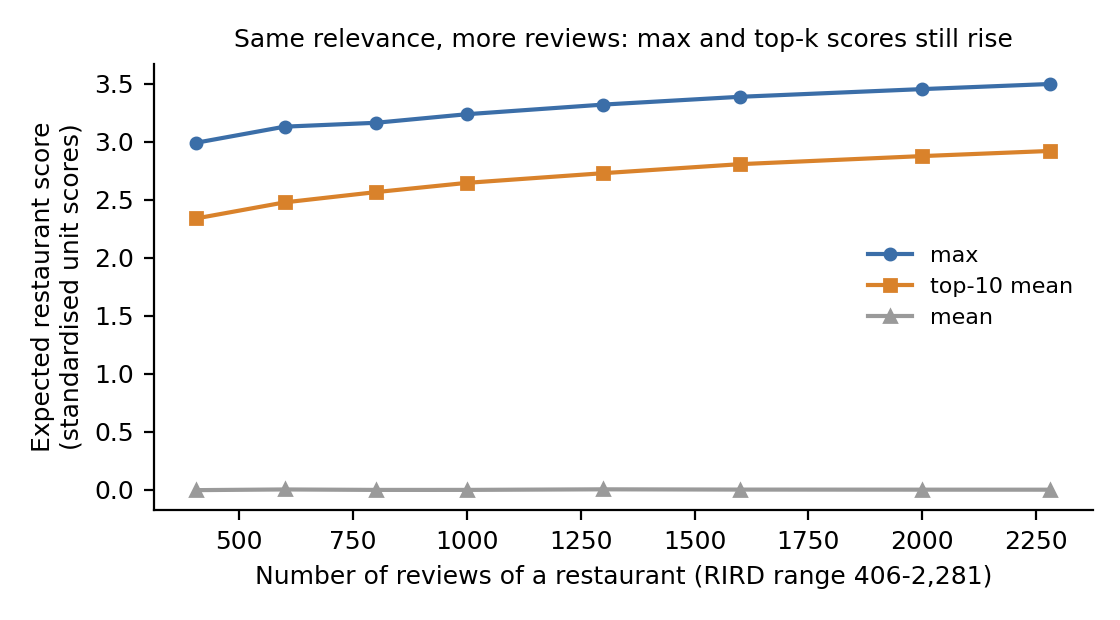
\includegraphics[width=0.78\linewidth]{figures/ch2_volume_simulation.png}
\caption{Simulation of the review-volume effect. Unit scores are drawn independently from a
standard normal distribution, identical for every restaurant (300 repetitions per point), so no
restaurant is more relevant than another. Generated by this project.}
\label{fig:volume-sim}
\end{figure}

\paragraph{Faithful and supportive evidence.} A good explanation must satisfy two different
conditions \citep{jacovi2020faithfulness}. It must be \emph{faithful}: the shown sentences must
be the real reason for the ranking. It must also be \emph{supportive}: a person reading the
sentence should agree that the restaurant fits the query. Figure~\ref{fig:intro-example} showed
a sentence that is likely faithful (it is the restaurant's highest-scoring unit) but not
supportive (it says
the restaurant is expensive). The two properties must be measured separately.

\paragraph{Thai.} Thai text must be segmented into sentences and words before BM25 can be
applied, and segmentation errors affect both retrieval and evidence. Thai taste requests often
contain negation, such as \thai{ไม่หวานมาก} (not too sweet), which is known to be difficult for
neural retrievers \citep{weller2024nevir}. Finally, no public Thai dataset links reviews to
restaurants and query labels, so Thai evaluation needs new human labels and can only be done at
sentence level.

\section{Research questions}
The guiding question from the proposal feedback is divided into three research questions:
\begin{description}
  \item[RQ1.] When BM25 and dense retrieval use identical units and aggregation, which method
  ranks restaurants better, and does the answer hold once review volume is controlled?
  \item[RQ2.] Do the shown review sentences faithfully reflect the ranking, and do human readers
  agree that they support the query?
  \item[RQ3.] Does sentence retrieval transfer to real Thai restaurant reviews, when evaluated
  with taste queries fixed in advance and human relevance labels?
\end{description}
Table~\ref{tab:rq-map} lists the data, measurement and metrics used for each question.

\begin{table}[H]
\centering\small
\caption{Research questions, the evidence used to answer them, and the data.}
\label{tab:rq-map}
\begin{tabularx}{\textwidth}{@{}p{1.1cm}p{2.0cm}LL@{}}
\toprule
RQ & Data & What is measured & Metrics and tests\\
\midrule
RQ1 & RIRD (English) & Restaurant ranking of BM25 vs.\ dense, review and sentence units, five
aggregations, with and without the 400-review cap & nDCG@5/10, MAP, MRR, P@k, R@k; bootstrap
95\% CIs; paired randomisation tests with Holm correction; score--count correlation\\
RQ2 & RIRD (English) & Effect of deleting the shown sentences vs.\ random sentences; human
0/1/2 support labels on shown sentences & Rank and nDCG drop; share of supporting sentences;
Cohen's $\kappa$\\
RQ3 & Wongnai (Thai) & Sentence ranking of BM25 vs.\ dense for 24 frozen taste queries, judged
on a pooled set of 452 pairs & nDCG@10, P@10; bootstrap CIs; paired randomisation test;
results by query type; Cohen's $\kappa$\\
\bottomrule
\end{tabularx}
\end{table}

\section{Expected outcomes}
For RQ1 we expected dense retrieval to beat BM25, because RIRD reports the same pattern for an
off-the-shelf dense model \citep{rird2023}; our contribution is to test it under a fair unit
control and a volume control. For RQ3 we did not assume the same pattern. On the Thai part of
the MIRACL benchmark, BM25 outperforms an older multilingual dense retriever
\citep{zhang2023miracl}, so either outcome was plausible. For RQ2 there was no prior
expectation: the example in Figure~\ref{fig:intro-example} already shows that evidence can be
faithful without being supportive.

\section{Scope and limitations}
\begin{table}[H]
\centering\small
\caption{What is inside and outside the scope of this project.}
\label{tab:scope}
\begin{tabularx}{\textwidth}{@{}LL@{}}
\toprule
In scope & Out of scope\\
\midrule
Restaurant ranking and explanations in English (RIRD) & Thai restaurant ranking (no restaurant
identifiers in Wongnai)\\
Sentence-level Thai retrieval with new human labels & Fine-tuning or training the encoder\\
Off-the-shelf BM25 and one multilingual dense encoder & Learned or rating-weighted fusion\\
Extracted review sentences as explanations & Generated explanations\\
LLM query rewriting and a cross-encoder in the live demo only & LLM query decomposition
\citep{korikov2024multiaspect}\\
\bottomrule
\end{tabularx}
\end{table}
The scope is deliberately narrow so that every claim in the report is backed by a measurement.
The main limitation is that the two tracks evaluate different steps: English results describe
restaurant ranking, Thai results describe sentence ranking, and the two sets of numbers cannot
be compared directly.
